\documentclass[11pt,a4paper]{article}
\usepackage[utf8]{inputenc}
\usepackage[english]{babel}
\usepackage{graphicx}
\usepackage{float}
\usepackage{amsmath}
\usepackage{hyperref}
\usepackage{booktabs}
\usepackage{geometry}
\usepackage{enumitem}
\geometry{margin=0.9in}
\setlist{noitemsep}

\title{\textbf{ToolWindow Usage Analysis Report}}
\author{Viktor Shishmarev}

\begin{document}

\maketitle

\section{Objective}

\textbf{Research Question:} Is there a statistically significant difference in tool window session duration between manual and automatic opening methods?
\\
\textbf{Dataset:} Event logs with 3,503 raw events tracking tool window activity (user ID, timestamp, event type, opening method).
\\
\textbf{Hypothesis:}
\begin{itemize}
    \item $H_0$: No difference in duration between manual and auto groups
    \item $H_1$: Significant difference exists between groups
\end{itemize}

\section{Methodology: Data Cleaning \& Anomaly Detection}

\subsection{The Challenge: Messy Real-World Data}

Raw event logs contained significant data quality issues (55\% anomalies):
\begin{itemize}
    \item Orphaned events (close without open, open without close)
    \item Duplicate opens, out-of-order timestamps
    \item Missing or invalid type values
    \item Unrealistic durations ($>$ 1 hour threshold)
\end{itemize}

\subsection{Our Approach: Smart Episode Reconstruction}

\textbf{Key Innovation:} User-level state machine for open/close event matching.
\\
\textbf{Algorithm:}
\begin{enumerate}
    \item \textbf{Load \& Validate}: Multithreaded CSV import to SQLite (producer-consumer pattern)
    \item \textbf{Sort by User}: Group events by \texttt{user\_id} and order chronologically
    \item \textbf{State Machine Matching}:
    \begin{itemize}
        \item Track current "open" state per user
        \item Match each "close" with corresponding "open"
        \item Detect anomalies: duplicate opens, missing pairs, timestamp violations
    \end{itemize}
    \item \textbf{Bifurcation}:
    \begin{itemize}
        \item \textbf{Clean episodes} $\rightarrow$ \texttt{clear} table (valid open-close pairs)
        \item \textbf{Anomalies} $\rightarrow$ \texttt{anomaly} table (with reason: \texttt{missing\_open}, \texttt{duplicate\_open}, \texttt{>duration}, etc.)
    \end{itemize}
    \item \textbf{Duration Calculation}: $\text{duration} = \frac{\text{close\_ts} - \text{open\_ts}}{60000}$ (minutes)
\end{enumerate}

\textbf{Result:} From 3,503 raw events $\rightarrow$ 1,574 clean episodes (617 manual, 957 auto)

\subsection{Statistical Testing}

\textbf{Mann-Whitney U Test:} Non-parametric comparison (no normality assumption, robust to outliers)
\\
\textbf{Cliff's Delta:} Effect size measurement
\[
\delta = \frac{\text{\#}\{x > y\} - \text{\#}\{x < y\}}{n_1 \cdot n_2}
\]
where $\text{\#}\{x > y\}$ = number of pairs where manual $>$ auto, $n_1, n_2$ = sample sizes
\\
Interpretation: $|\delta| \geq 0.47$ = large effect

\section{Results}

\subsection{Data Processing Summary}
\begin{itemize}
    \item Raw events: 3,503 $\rightarrow$ Clean episodes: 1,574 (45\% retention)
    \item Anomalies filtered: 1,929 (55\%) — demonstrates importance of cleaning methodology
    \item Manual episodes: 617 | Auto episodes: 957
\end{itemize}

\subsection{Descriptive Statistics}

\begin{table}[H]
\centering
\begin{tabular}{@{}lrr@{}}
\toprule
\textbf{Metric} & \textbf{Manual} & \textbf{Auto} \\
\midrule
Count & 617 & 957 \\
Median (min) & \textbf{0.20} & \textbf{2.67} \\
Mean (min) & 10.52 & 27.85 \\
Q1 - Q3 (min) & 0.04 - 2.22 & 0.53 - 15.23 \\
Std Dev (min) & 50.17 & 79.18 \\
\bottomrule
\end{tabular}
\caption{Duration Statistics by Opening Type}
\end{table}

\subsection{Statistical Significance}

\begin{table}[H]
\centering
\begin{tabular}{@{}ll@{}}
\toprule
\textbf{Test} & \textbf{Result} \\
\midrule
Mann-Whitney U & 151,898.50 \\
p-value & $< 0.001$ \textbf{(highly significant)} \\
Cliff's Delta & $-0.4855$ \textbf{(large effect)} \\
Conclusion & \textbf{Reject $H_0$} \\
\bottomrule
\end{tabular}
\caption{Statistical Test Results}
\end{table}

\textbf{Interpretation:} Manual durations are significantly and substantially lower than auto durations.

\subsection{Visualizations}

\begin{figure}[H]
    \centering
    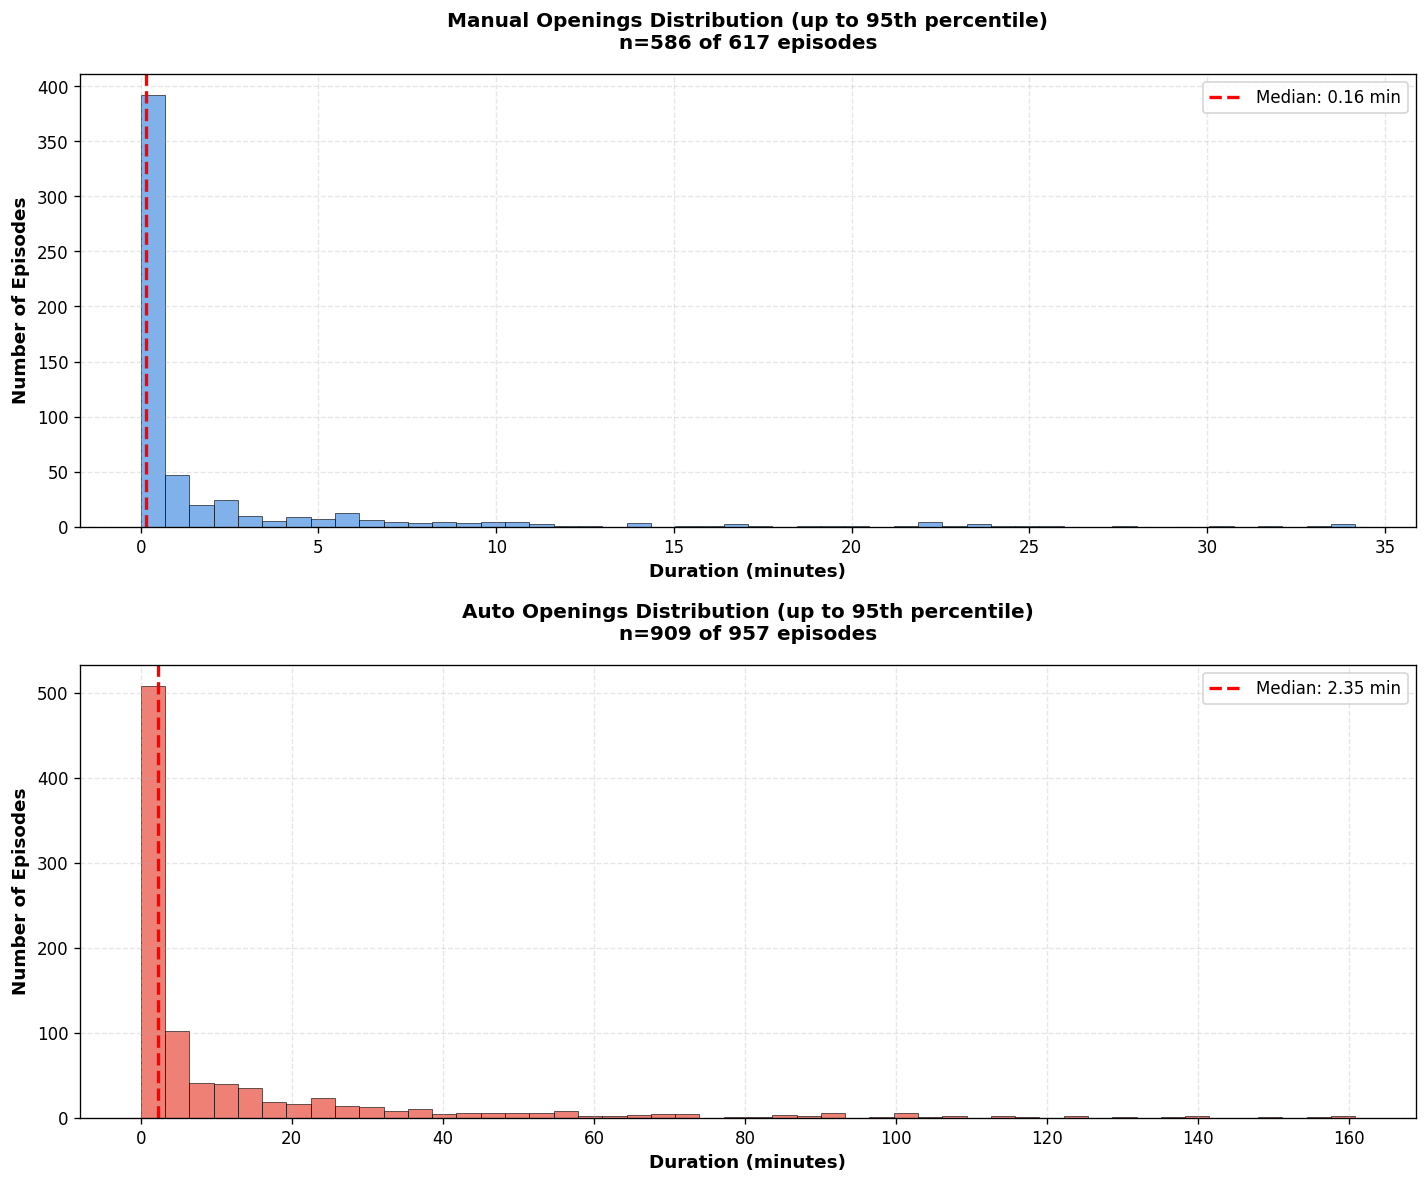
\includegraphics[width=0.7\textwidth]{plots/histogram.png}
    \caption{Duration Distribution Comparison}
\end{figure}

\begin{figure}[H]
    \centering
    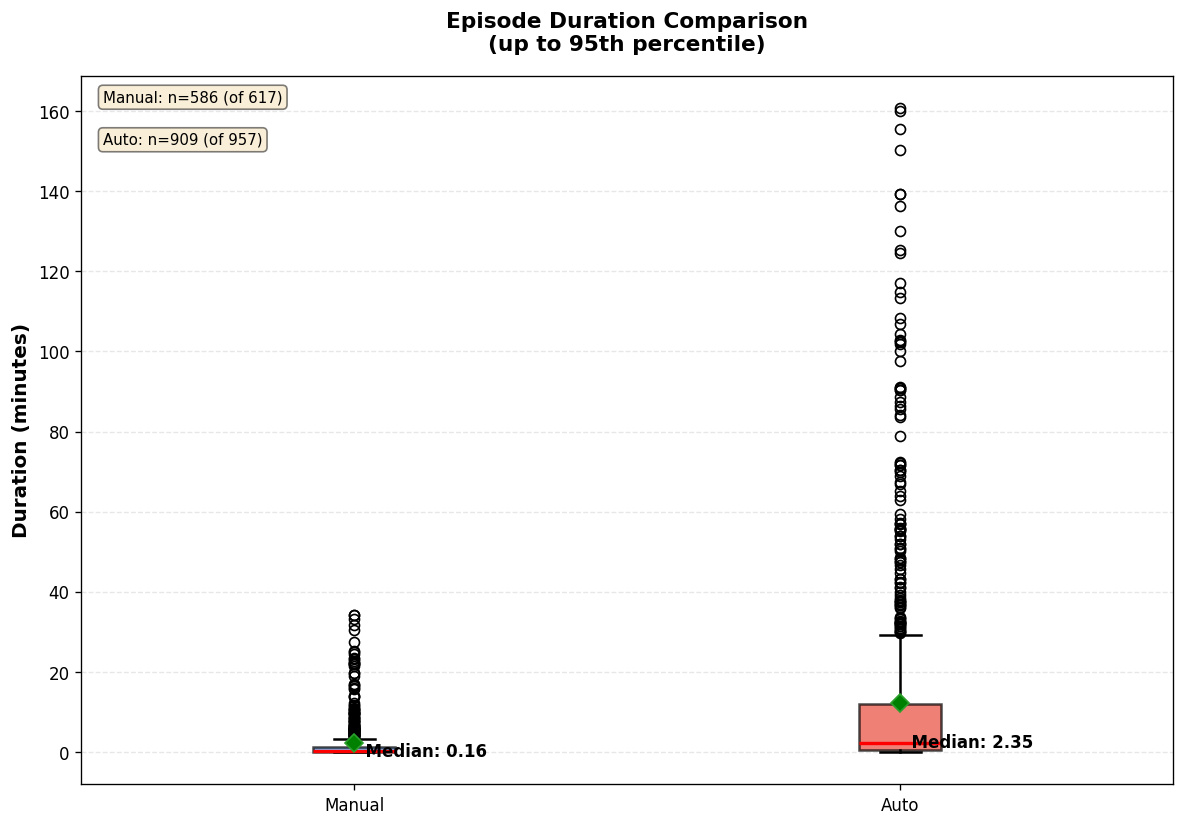
\includegraphics[width=0.7\textwidth]{plots/boxplot.png}
    \caption{Box Plot: Quartiles and Outliers}
\end{figure}
\newpage
\section{Key Insights}

\subsection{Main Finding}
\textbf{Manual openings are 13× faster to close (median):} 0.20 min vs 2.67 min
\\
\textbf{Why?}
\begin{itemize}
    \item \textbf{Manual}: Task-focused, quick information lookup $\rightarrow$ close immediately
    \item \textbf{Auto}: Workflow-integrated (debugging, testing) $\rightarrow$ stay open during entire task
\end{itemize}

\subsection{Methodological Success}
\begin{itemize}
    \item Without state-machine matching, analysis would be impossible
    \item Bifurcation strategy (clean vs anomaly tables) ensures data integrity
    \item User-level processing prevents cross-contamination
\end{itemize}

\section{Conclusions}

\begin{table}[H]
\centering
\begin{tabular}{@{}p{0.3\textwidth}p{0.65\textwidth}@{}}
\toprule
\textbf{Question} & \textbf{Answer} \\
\midrule
Significant difference? & \textbf{YES} — p $< 0.001$, large effect ($\delta = -0.4855$) \\
Practical impact? & \textbf{Manual 13× faster to close} (0.20 vs 2.67 min median) \\
Business insight? & Manual = quick lookup; Auto = workflow integration \\
\bottomrule
\end{tabular}
\end{table}


\vspace{1em}
\hrule
\vspace{0.5em}

\noindent\textbf{Technology Stack:} Python 3.12+ | SQLite3 | scipy | matplotlib | FastAPI | Docker

\noindent\textbf{Repository:} \url{https://github.com/shishmarevv/ToolWindowData} | \textbf{Reproducible:} \texttt{make all}

\end{document}